\documentclass[11pt]{jsarticle}

\title{デザインパターン入門 レポート}
\author{平川 一樹}
\date{\today}

\usepackage[top=30truemm,bottom=30truemm,left=25truemm,right=25truemm]{geometry}

\usepackage{listings}
%\begin{lstlisting}[basicstyle=\ttfamily\scriptsize, frame=single] 

\usepackage{color}
\usepackage[dvipdfmx]{graphicx}
\usepackage{mediabb}


\graphicspath{{./image/}}

%図表番号のつけ方を変更
\makeatletter
	\renewcommand{\theequation}{% 式番号の付け方
	\thesection.\arabic{equation}}
	\@addtoreset{equation}{section}

	\renewcommand{\thefigure}{% 図番号の付け方
	\thesection.\arabic{figure}}
	\@addtoreset{figure}{section}

	\renewcommand{\thetable}{% 表番号の付け方
	\thesection.\arabic{table}}
	\@addtoreset{table}{section}
	
	\@addtoreset{footnote}{section}%セクションごとにFootNoteカウンタをリセット
\makeatother

\begin{document}
	\maketitle
	
	\begin{abstract}
		2018年3月30日から作成開始。
		
		デザインパターンの学習を目的にレポートを書いていく。
		3日坊主にならないように気をつけよう\verb|^^|
		
		このレポートは「Java言語で学ぶ デザインパターン入門」(図\ref{fig::book}参考)を元に作っている。
		本を読んで理解した後、なるべく本を見ずに概要・例・考察・疑問点を書いて理解を確認する形式で進めていこうと思う。
		
		1日の終わりには感想をまとめておく。
		\begin{figure}[htbp]
			\centering
			\includegraphics[width = 5cm, bb = 0 0 199 253]{book.jpg}
			\caption{参考文献}\label{fig::book}
		\end{figure}
	\end{abstract}
	
	\clearpage
	\tableofcontents
	\clearpage
	
	\section{Iteratorパターン}
	\subsection{概要}
		あるコレクションの要素に便利にアクセスするためのデザインパターン。
		
		イテレータクラスを作り、コレクションを持つクラスがイテレータクラスを返すようにする事で、
		後はイテレータクラスのみを用いてコレクションにアクセスできる。
		
		イテレータクラスとイテレータを返すクラスはインターフェースを用いて実装するべきメソッドを定めておく。
	\subsection{例}
		図\ref{fig::iterator}はIteratorパターンの一例だ。
		Aggregate、Iteratorというインターフェースを作り、
		それらを実装する事でIteratorパターンを実現している。
		
		ConcreteIteratorはConcreteAggregateが持っているコレクションなどにアクセスする。
		Nextはコレクションの要素を返して、参照を次に移動するメソッド、
		hasNextは次の参照を持っているかどうか\footnote{コレクションの最後の参照かどうかとも言い換えられる}
		を判断して返すメソッドとなっている。
	
		\begin{figure}[htbp]
			\centering
			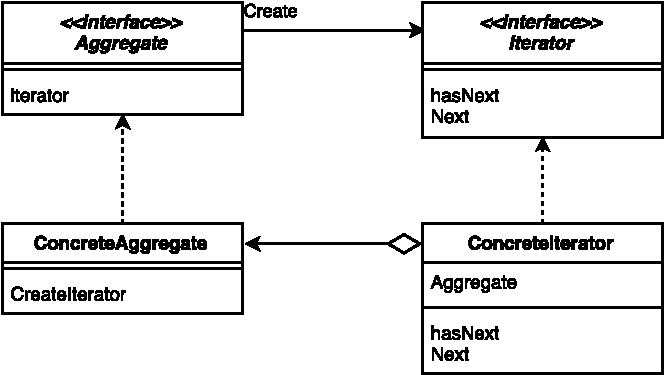
\includegraphics[width=0.7\hsize]{IteratorPattern-crop.pdf}
			\caption{(例)Iteratorパターン}\label{fig::iterator}
		\end{figure}
		
	\subsection{考察}
		C++のIteratorと同じようなものかと思ったが、それは今回のパターンとは少し実装の仕方が違っている気がした。
		特にC++はインターフェースを使っておらず、Iteratorクラスの定義が、Aggregateクラスの中に書かれていた覚えがある。
		C\#のIEnumerableとIEnumeratorがこのパターンを使っているのだろうと感じた。
		
		自分でこのパターンを使ったこともあったが、
		その時はインターフェースを作らずに直接Iteratorクラスを作ってしまった。
		その結果、Iteratorクラスの内容はかなり独特なものになってしまったと思う。
		インターフェースを用いた方が、例でいうConcreteクラスの内容がどうであれインターフェースの
		様式\footnote{今回の例ではhasNext、nextのメソッドを知っているだけで使える}
		のみを知っていれば扱えるようになるのがかなりのメリットだと感じた。
	\subsection{疑問点}
		特になし。
	\section*{\textcolor{blue}{2018年3月30日時点のコメント}}
		\subsection*{\textcolor{blue}{感想}}
			レポートを書こうと思い立って1日目が終了。
			
			\TeX の環境を構築したり、クラス図を作るための手段を調べるのに時間がかかってしまい、
			今回は1つのデザインパターンしか書けなかったが今後はもう少し早いペースで書いていけると思う。
			
			Iteratorパターンも読み始める前はわかっているつもりだったが、読んでみるとなかなか有益だったと思う。
			\clearpage
			
	\section{Adapterパターン}
		\subsection{概要}
			あるクラスの振る舞いを他のクラスを用いて作り変えるようなイメージを持っている。
			
			既に提供されているクラスを自分が必要としているクラスに作り変えて、
			提供されている機能と必要としている機能のズレを修正できる。
			
			例えば、全言語対応の翻訳を行うクラスなどが提供されているとする。
			しかし、今必要なのは日本語と英語の翻訳機能だけだと言った場合に、
			このパターンを使ってシンプルな振る舞いのクラスに作り変えることができる。
			
			出てくる用語としては以下の3つがある。
			
			\begin{description}
				\item[Target]現在の環境で必要な振る舞い
				\item[Adaptee]適合される対象
				\item[Adapter]適合させるクラス
			\end{description}

			
			このパターンの実現には以下の2通りの実現方法がある。
			\begin{itemize}
				\item{継承を用いる}
				\item{委譲を用いる}
			\end{itemize}
			
			\subsubsection{継承を用いる実現方法}
				まずどのような機能が欲しいかをTargetインターフェースに定めておき、
				Adapteeを継承し、Targetを実装したAdapterクラスを作る。
				後は、
				\begin{lstlisting}[basicstyle=\ttfamily\scriptsize, frame=single] 
Target obj = new Adapter();
				\end{lstlisting}
				というイメージで、Adapteeの存在は無いものとして使用していく。
				
			\subsubsection{委譲を用いる実現方法}\label{sec::adapter1}
				AdapterクラスにAdapteeクラスのデータを持たせる。
				TargetクラスはAdapterを継承する。使う側はTargetクラスを使用していく。
		\subsection{例}\label{sub::adapter1}
			様々な動物の鳴き声音声を管理するAnimalVoiceクラスが提供されていたとする。
			しかし、実際にはクイズアプリを作っていて、
			正解の場合に犬の鳴き声、間違いの場合は猫の鳴き声を取得したいものとする。
			
			\begin{figure}[htbp]
				\centering
				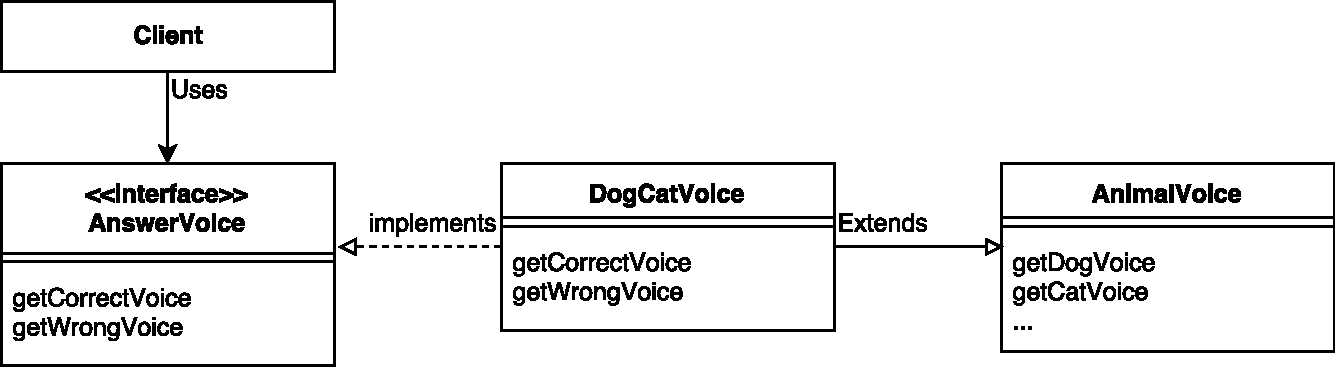
\includegraphics[width = 0.8\hsize]{AdapterPattern1.pdf}
				\caption{継承によるAdapterパターン}\label{fig::Adapter1}
				
				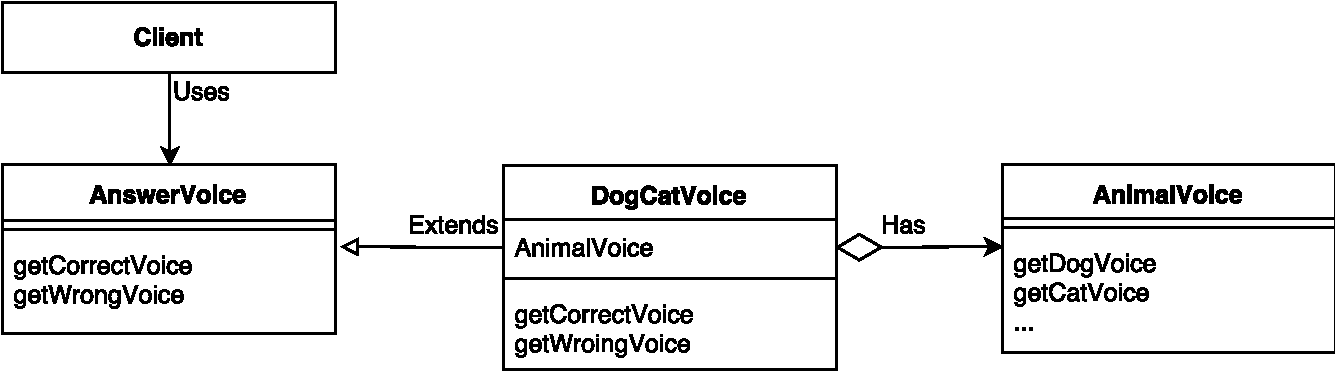
\includegraphics[width = 0.8\hsize]{AdapterPattern2.pdf}
				\caption{委譲によるAdapterパターン}\label{fig::Adapter2}
			\end{figure}
			
			図\ref{fig::Adapter1}と図\ref{fig::Adapter2}はそれぞれ、継承・委譲によるAdapterパターンで作成している。
			
			TargetがAnswerVoice、AdpterがDogCatVoice\footnote{命名が少し不安$\cdots$少し命名の仕方が違うような気がする}
			と割り当てている。
			この方法で作成すれば、使用者ClientはAnimalVoiceの仕様を理解していなくてもコードが書け、
			メソッド名もgetCorrectVoiceのように、現在のプロジェクトに適したメソッド名に置き換えることができる。
		
		\subsection{考察}
			Adapterパターンは今までよく使っていたが、今回学んだ設計方法とは少し異なっていた。
			特に、Targetの概念を無視して作っていたと思う。今まではAdapterを直接使用するイメージだ。
			C言語ライブラリをC++でクラスのように扱うというような場合は今までの方法で良かったのかもしれないが、
			今後はTargetの存在も意識しながらAdapterパターンを使っていこうと思う。
			
		\color{red}
		\subsection{疑問点}
			\subsubsection{Adapterの使用範囲}
				どのぐらいまでAdapterパターンを使った方が良いのかが疑問になっている。
				例えば、IOSのUIButtonクラスなどをAdapterするのは少々やり過ぎなイメージがある。
				自分に分かりやすいメソッドをいくら定義しても、
				周りからは新しいクラスを覚える必要性が生じるので、
				見づらく感じてしまうのでは無いか?と思う。
				
				しかし、マイナーなライブラリを使っている場合などに、
				今の環境に適したメソッド名をつけたりしながら、
				分かりやすいクラスに作り変えていく方法なら積極的に活用するべきだとも思う。
				
				どのぐらいの範囲でAdapterパターンを使っていくのかが
				現在の疑問点だ\footnote{それを経験で養うのかもしれないが$\cdots$}。
			\subsubsection{TargetとAdapterを分ける理由}
				Targetをインターフェースなどで定めなくとも、Adapterクラスを使用すれば解決するのでは無いか?という
				疑問も少し浮かんだ。
				
				節\ref{sub::adapter1}の継承を使用した例で言うなら、後で仕様が変わった場合などに、
				Targetインターフェースを実装した新たなAdapterクラスを作ることで、
				正解なら像、不正解ならライオンみたいな実装に容易に変えることができるからなのか?
				という感じで現在のところは理解している。
		\color{black}
		
	\section*{\textcolor{blue}{2018年3月30日時点のコメント}}
		\subsection*{\textcolor{blue}{感想}}
			レポートを書こうと思い立って2日目が終了。
			
			今回は、ソースツリーを用いて、このレポートの環境をGitHubのリポジトリにプッシュしてみることにして見た。
			ソースツリーの外観に慣れてみるのと、レポートを公開できる環境にしたかったからだ。
			レポートはPDF形式なので、差分の恩恵は受けられないと思うが、\TeX のコードは差分が見れるかもしれない。
			
			勤務日だったのもあり、前回同様1つのデザインパターンしか書けなかったが、この調子で進めていこう。
			\clearpage
			
	\section{Template Methodパターン}
		\subsection{概要}
			処理の大まかな流れを定めて、
			細かな処理は子クラスに任せるようなイメージを持っている。
			
			親クラスでいくつか抽象メソッドを作っておき、
			その抽象メソッドを使って、別のメソッドの内容を定義する。
			その親クラスは抽象クラスとなるが、
			継承を用いて抽象メソッドの実装を行うことで、全てのメソッドが使用可能となる。
			
		\subsection{例}
			図\ref{fig::TemplateMethod1}はTemplateMethodパターンの一例を考えたものだ。
			Productsクラスは商品を扱うクラスで、
			商品の価格と数量から合計金額をgetPrizeメソッドで計算出来るようにする。
			
			Product1〜3のクラスはProductsクラスを継承し、
			getUnitPrizeという商品単価をもとめるメソッド、
			getNumberという商品の個数をもとめるメソッドをオーバーライドする
			\footnote{実際にはメソッドよりプロパティにするべきかもしれない。
			このパターンにする必要性はあまり感じないかもしれないが、
			Product1はネットから、Product2はHDから、といったように情報の取得方法が違う場合を想定している。}。
			
			このようにすることで、Product1〜3のgetPrizeはそれぞれ適切な方法で単価と数量を取得し、
			合計金額を計算するgetPrizeメソッドを適切な方法で計算させることができる。
			
			\begin{figure}[htbp]
				\centering
				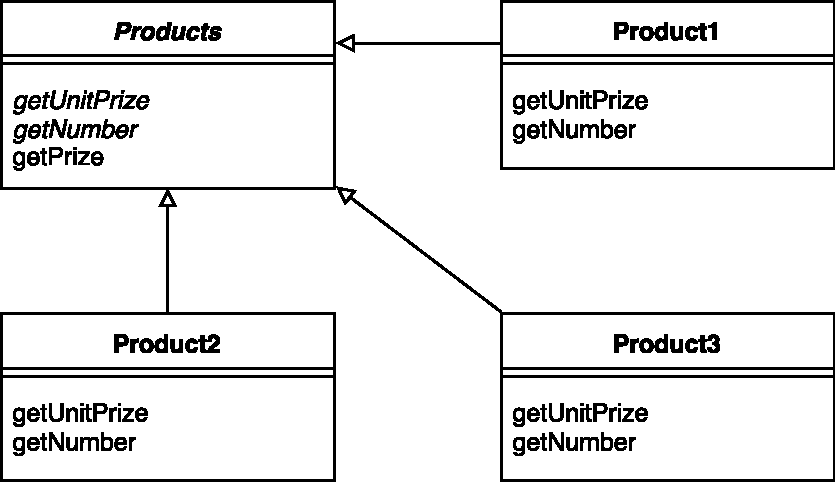
\includegraphics[width = 0.5\hsize]{TemplateMethodPattern.pdf}
				\caption{TemplateMethodパターンの一例}
				\label{fig::TemplateMethod1}
			\end{figure}
			
		\subsection{考察}
			このパターンは何回か使ったことがあったが、
			あまり積極的に使ったことは無かった。
			
			複数のクラスに継承される親クラスを作る場合は常にこの考え方を念頭に入れるべきだと思った。
			「何か似ているクラスを作っているな〜」と感じた時にもこのパターンを視野に入れて作ってみたい。
		
		\color{red}
		\subsection{疑問点}
			特になし
		\color{black}
		
		\section*{\textcolor{blue}{2018年4月4日時点のコメント}}
		\subsection*{\textcolor{blue}{感想}}
			最近忙しくてなかなか手がつけられていなかったが、
			今日はなんとか1章進めることができた。
			
			FactoryMethod、Singletonなど
			2章先ぐらいまでは読んでいるが、
			レポートの方が遅れ気味なので追いつきたい。
			\clearpage
			
		\section{FactoryMethodパターン}
			\subsection{概要}
				あらかじめ抽象クラスを用いて、作成者と製品を作る。
				
				この際、作成者クラスには製品クラスを作成するためのメソッド(ここではCreate)を設ける。
				Createメソッド自体を抽象メソッド
				\footnote{抽象ではなく仮装メソッドとして、デフォルトの処理を書いておいても良い。}
				として子クラスに実装を任しても良いが、
				Createメソッドの中身が複雑な場合にTemplateMethodパターンを用いて、
				子クラスに実装を任すことで、
				インスタンスの作成方法を一般化することができる。
				
				製品クラスは抽象クラスとし、製品の振る舞いを抽象メソッドで定めておく。
				
				あとは、この2つのクラスを継承し、具体的な作成者クラス、具体的な製品クラスを作っていく。
				
			\subsection{例}
				シューティングゲームなどに用いられる弾やレーザーなどのオブジェクトを管理する際などに、
				このパターンを用いることを例に挙げていく。
				弾の作成にはルールがあり、1秒以内に複数の弾は作成できないものとする。
				つまり、一度弾を作ると1秒間新しい弾は作れないものとする。
				ただ、レーザーについては3秒間に1回とする。
				
				クラス名については以下のように定める\footnote{もう少し良い命名があったとは思うけど...}。
				コードは図\ref{fig::factoryMethod1}の様になった。
				\begin{description}
					\item[Factory]{作成者クラス}
					\item[Product]{製品クラス}
					\item[BulletFactory]{弾の作成者クラス}
					\item[Bullet]{弾の製品クラス}
					\item[LaserFactory]{レーザーの作成者クラス}
					\item[Laser]{レーザーの製品クラス}
				\end{description}
				
				このように作ることで、
				何秒間に1回までしか作成できないという決まりごとを定めることができる。
				また新しく爆弾オブジェクトを作ることになった場合でも、
				時間確認の処理の実装を忘れることはない。
				
				\begin{figure}[htbp]
					\centering
					\begin{lstlisting}[basicstyle=\ttfamily\scriptsize, frame=single] 
abstract class Factory{
	private Time beforeTime;
	
	public Product create(Point pt){
		Time now = Now();
		bool judge = judgeCreate(now - beforeTime);
		beforeTime = now;
	
		if(judge){
			return createProduct(pt);
		}else{
			return null;
		}
	}
	
	public abstract Product createProduct(Point pt);
	public abstract bool judgeCreate(Time tm);
}

class BulletFactory : Factory{
	public override Product createProduct(Point pt)(
		return new Bullet(Point pt);
	}
	
	public override bool judgeCreate(Time tm){
		return tm.toSecond() >= 1.0;
	}
}

class LaserFactory : Factory{
	public override Product createProduct(Point pt){
		return new Laser(Point pt);
	}
	
	public override bool judgeCreate(Time tm){
		return tm.toSecond() >= 3.0;
	}
}

abstract class Product{
	...
}

class Bullet : Product{
	public Point centerPoint;
	public Bullet(Point pt){
		centerPoint = pt;
	}
	
	...
}

class Laser : Product{
	...
}
					\end{lstlisting}
					\caption{FactoryMethodパターンの一例}
					\label{fig::factoryMethod1}
				\end{figure}
			
			\subsection{考察}
				このデザインパターンはまだ使ったことがなかった。
				TemplateMethodパターンに似ているが、
				作成方法の枠組みを定めているところが前回との違いだと思う。
				
				インスタンスの作成方法から振る舞いまで酷似しているようなクラスを設計する場合には、
				このパターンを使うことになるのかもしれない。
			
			\color{red}
			\subsection{疑問点}
				\subsubsection{製品クラスの設計}
					今回の例では、内容について省略させてもらったが、
					製品クラスに振る舞い(つまりメソッド)のみしか記入しないのであれば、
					インターフェイスを使うこともできるのではないか、という疑問が残った。
					
					製品クラスを継承するような事例がないのでどちらでもいいのかもしれない。
					もしくは製品クラスに変数を持たせる必要が出てくる場合もあるのかもしれない。				
			\color{black}
			
	\section{Singletonパターン}
		\subsection{概要}
			プログラム上であるクラスのインスタンスが必ず1つしか存在しないことを保証するためのデザインパターン。
			
			クラスのフィールドに自分自身を保持する静的メンバを持ち、メソッドでその変数を返せるようにする。
			変数、コンストラクタはprivateとし、クラス外から新しいインスタンスは作らせないようにする。
			
		\subsection{例}
			図\ref{fig::Singleton1}はメソッドを呼ぶたびに、$1\cdot 2\cdot 3\cdots$と数値を返す例だ。
			
			\begin{figure}[htbp]
				\centering
				\begin{lstlisting}[basicstyle=\ttfamily\scriptsize, frame=single] 
class CountNumber{
	private num = 0;

	private static CountNumber singleton = new CountNumber();
	
	private CountNumber() { }
	
	public CountNumber Singleton{
		get{
			return singleton;
		}
	}
	
	public getCount(){
		return ++num;
	}
}
				\end{lstlisting}
				\caption{Singletonパターンの一例}
				\label{fig::Singleton1}
			\end{figure}
			
		\subsection{考察}
			このパターンについては聞いたことがあるだけのレベルで、
			実際どんな時に使えば良いかは考えたことがなかった。
			
			しかし、前章のFactoryMethodパターンの製作者クラスをSingletonパターンで実装することは
			有効なのではないかと思った。
			
		\color{red}
		\subsection{疑問点}
			\subsubsection{静的クラスとの使い分け}
				Singletonパターンと静的クラスは非常によく似ていると思う。
				
				静的クラスは継承出来ないので、FactoryMethodパターンなどに応用する場合は、
				Singletonパターンを使うべきだと思う。
				
				しかし、使い分けの基準が継承できるかどうかだけなのかはまだ疑問な部分。
				Singletonは引数に出来る...という理由も考えたが、
				そもそも一つしかインスタンスはないのだから引数にする理由もあまりない気がしている。
		\color{black}
			
		\section*{\textcolor{blue}{2018年4月6日時点のコメント}}
			\subsection*{\textcolor{blue}{感想}}
			今日はFactoryMethodパターン、Singletonパターンの2章を書いた。
			
			FactoryMethodはなかなか複雑で例を考えるのに苦労したが、
			慣れればとても有用なパターンだと思った。
			
			全23章なので$20\%$ほど終わったところ。
			次はPrototypeパターン。なにやらインスタンスを作成する方法らしいので、
			FactoryMethodと同じような分類なのか。
			今後もこの調子で進めていこう。
			\clearpage	
			
			
			
			
			
			
			
			
		
\end{document}